\chapter{基于纯视觉的体积测算方法研究}
\label{cha:chap4}
\section{引言}
\label{sec:4.1}
利用三维重建的技术流程,可以通过输入二维图片序列的方式获取到场景中的三维稀疏点云或者稠密点云,以视觉的方式来表达场景中的信息。
虽然这些点云可以描绘出空间中的信息,但是还存在以下两个这些问题需要解决:

1)	在三维重建的过程中,由于点云坐标系都是以第一帧的相机为参考坐标系,因此点云坐标系和真实世界坐标系无法对应,对于很多实际应
用场景,都需要获取到该场景的实际水平面,来进行下一步的导航和定位;

2)	由于是单目相机,无法获取特征点的深度信息,因此对于构建出的三维重建点云没有一个绝对尺度的概念。

在解决上述两个问题的基础上,可以对空间中的封闭物体进行高度,面积或者体积的测算,对比传统方法中用激光雷达等设备来测算体积的方
式,现在就可以通过单个摄像头以纯视觉的方式来完成上述过程,并获取到一个精确的结果。本章将以三维重建的点云结果为基础,为了解决
点云的尺度问题,以及求解三维点云的水平面方程,本文将在场景中引入Aruco二维码,因为Aruco二维码本身携带尺度信息,每一种二维码
都有唯一的ID值,并且其还具备较为容易检出的角点坐标。在获取到尺度和水平面方程后,随后结合点云信息可以再进一步计算三维场景的体
积,具体流程如图~\ref{fig:getVolume}所示。

\begin{figure}[H] % use float package if you want it here
    \centering
    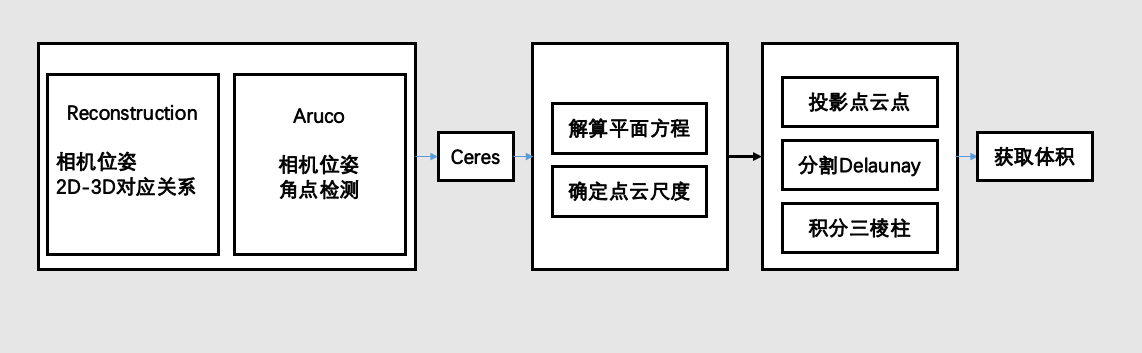
\includegraphics[height=5cm]{getVolume.png}
    \caption{体积测算流程图}
    \label{fig:getVolume}
  \end{figure}

\section{解析水平面方程的一般方法}
\label{sec:4.2}
\subsection{检测2D点坐标}
\label{sec:4.2.1}
对于大尺度的场景,都需要得到该场景的水平面所在的平面的方程,一方面由于物体的遮挡,水平面很难直接通过视觉的方法构建出来,从而
导致整个场景非闭合,因此添加水平面后可以使得整个场景封闭;另一方面,水平面的存在能够更好的计算场景的几何特性,例如场景的高度,
面积,体积等。由于三维重建本身的点云结果都是基于参考坐标系,没有和世界坐标系对齐,本文考虑到可以结合点云中能够获取到世界坐标
系的Aruco二维码作为媒介,进行坐标系的转换。

如图~\ref{fig:getVolume_Aruco_detect}所示,可以检测出场景中二维码的ID值,位置,大小,角点坐标等信息,因为在场景中,
Aruco二维码的布置都会有下侧两个角点直接落在水平面上,因此可以认为所有二维码的下侧角点所构成的平面即是场景的水平面。那么接下
来即可将水平面的求解转化为二维码角点所在平面的求解。在检测的过程中,需要将所有2D图片的索引和角点的位置记录下即可。

\begin{figure}[H] % use float package if you want it here
\centering
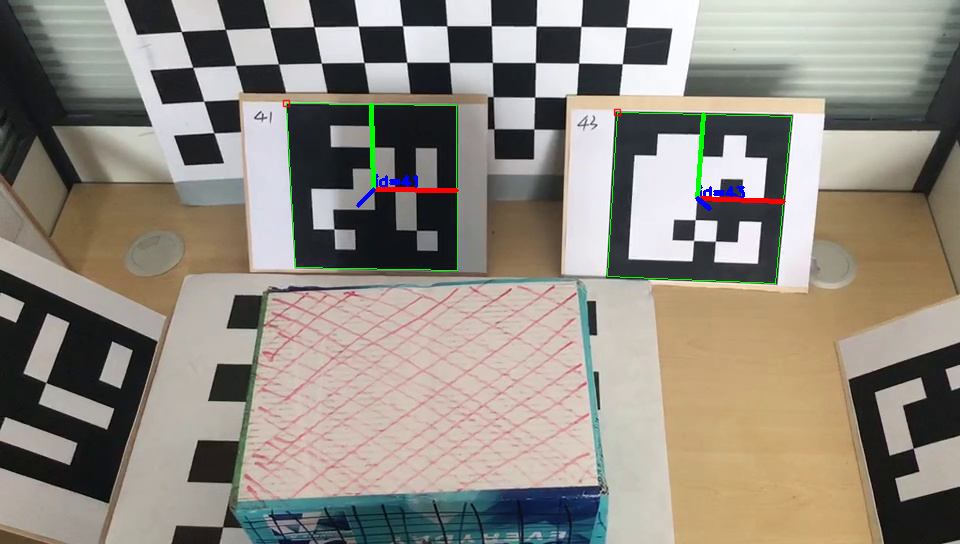
\includegraphics[height=8cm]{getVolume_Aruco_detect.png}
\caption{Aruco二维码检测示意图}
\label{fig:getVolume_Aruco_detect}
\end{figure}

\subsection{寻找对应3D坐标}
\label{sec:4.2.2}
在上一小结中,可以获得连续视频帧中每一帧的Aruco二维码下侧两个角点的坐标值,同样的,可以直接将如图~\ref{fig:getVolume_inputCamera}
所示的这些包含二维码的视频帧序列作为三维重建的输入以获取场景的点云,考虑到Aruco的角点被作为特征点时极易被检出,因此只需要通
过稀疏点云,即可获取角点在二维图像中的坐标和三维重建点云中的三维坐标之间的对应关系。

\begin{figure}[H] % use float package if you want it here
  \centering
  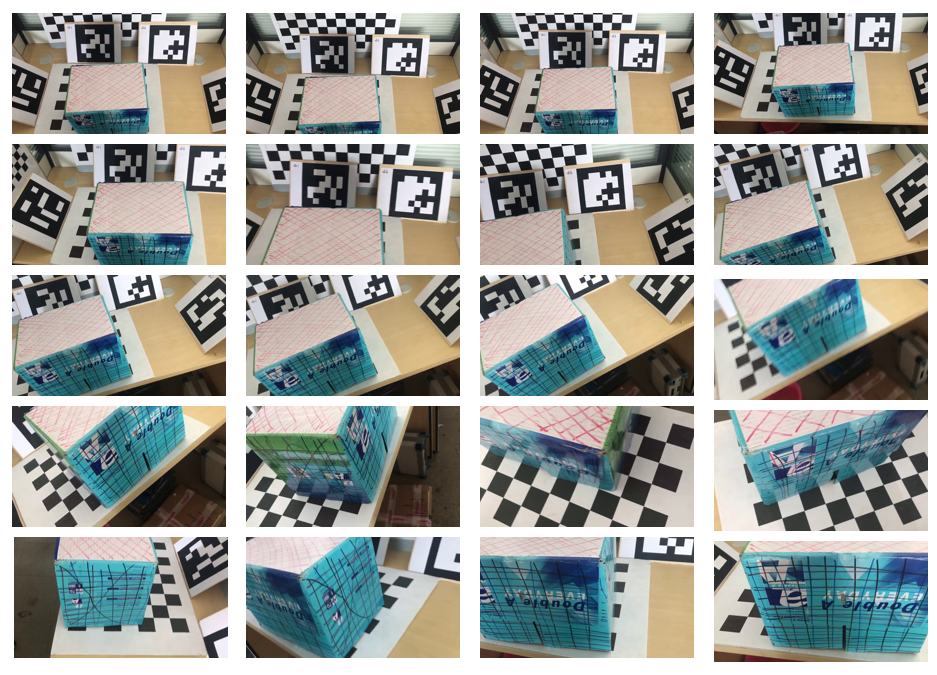
\includegraphics[height=9cm]{getVolume_inputCamera.png}
  \caption{三维重建输入视频序列图}
  \label{fig:getVolume_inputCamera}
  \end{figure}
在三维重建的过程中,可以获取到每一帧图像中所有特征点所对应的三维重建点云中的三维坐标,无论是稠密点云或者稀疏点云,都可以得到
一个对应关系,但是考虑到遍历的效率问题,则选择稀疏点云中的点击作为遍历对象。在寻找对应关系的实际过程中,会遇到二维坐标无法映
射到三维坐标点的情况,那么则会优先选择距离二维点坐标欧氏距离最近的点作为替代对象。此外,还需要注意的是,若所布置的Aruco二维
码的所有下侧点都位于同一条直线上,那么这样就无法获取准确的水平面方程,因为经过同一直线的平面并不唯一,因此在布置坐标的过程中
需要注意将所有Aruco二维码尽可能对立放置。
\section{结合opencv解算平面和尺度}
\label{sec:4.3}
内容内容内容内容内容内容内容内容内容内容内容内容内容内容内容
\section{解算体积}
\label{sec:4.4}
内容内容内容内容内容内容内容内容内容内容内容内容内容内容内容

